\documentclass{article}

\usepackage{hyperref}
\usepackage[a4paper, margin=1in]{geometry}
\usepackage{cite}
\usepackage{upquote}
\usepackage{tikz}
\usepackage{textcomp}

\tikzstyle{plain} = [rectangle, rounded corners, text centered, draw=black]
\tikzstyle{trusted} = [rectangle, rounded corners, text centered, draw=black, fill=red!20]
\tikzstyle{untrusted} = [rectangle, rounded corners, text centered, draw=black, fill=yellow!20]
\tikzstyle{arrow} = [thick,->,>=stealth]

\title{Kerberos-based single sign-on with delegation for web applications}
\author{Daniel Carter}
\date {\today}

\begin{document}
\maketitle

\section{Introduction}

\subsection{Web application security}
Many web applications are built around a database, which is used by the application framework to store user data and load it for display to the user. In general, the user logs in using a username and password (which is checked by the web app framework itself), and the application then makes database queries on the user's behalf, processes the results, and displays them to the user in a suitable way.

In this scenario, the application framework has the ability to read and write arbitrary data in the database, and the only thing which prevents a malicious user from accessing data which they are not authorised to read is the application code itself. This is potentially problematic, since web app authors are often not security experts and may accidentally cause data to be visible to the wrong users. Some examples of how this can occur include:

\begin{itemize}
\item
  \textbf{SQL injection}, a form of command injection attack (which are currently number 1 in the OWASP \textit{Top 10 Web Application Security Risks} list\cite{OWASP10}). This occurs when an application uses a template database query such as
\begin{verbatim}
SELECT * FROM records WHERE username='$user';
\end{verbatim}
and replaces \verb+$user+ with a string that the user provides. However, with insufficient checking of parameters, a user can supply a string such as
\begin{verbatim}
' OR 1=1; --
\end{verbatim}
resulting in a total query of
\begin{verbatim}
SELECT * FROM records WHERE username='' OR 1=1; --';
\end{verbatim}
which returns the records of all users (since \verb+1=1+ is always true).

\item
  \textbf{Master password leakage}, which enables any user to arbitrarily read and write from the database. Since the web app itself has these capabilities, it usually has a single username and password which it uses to authenticate with the database, and these are usually stored in a simple configuration file. If the webserver is misconfigured such that the configuration file is visible over the internet, or if the file is accidentally checked into a public source control repository, an attacker can read this file, connect to the database server and read out all the data.

\end{itemize}

As well as being commercially and reputationally damaging, unauthorised access to data can result in severe legal penalties: the Data Protection Act 2018 specifies a fine of up to 2\% of a company's global turnover (or 10 million Euros, if that is greater) may apply in cases of unauthorised disclosure of personal data\cite{GDPR}. Developing technologies that mean the web app does not have to be trusted with all data can significantly reduce the risk of these types of disclosure.

The following diagram represents an example of a typical current setup, and the problems that can be caused if an SQL injection vulnerability is present:

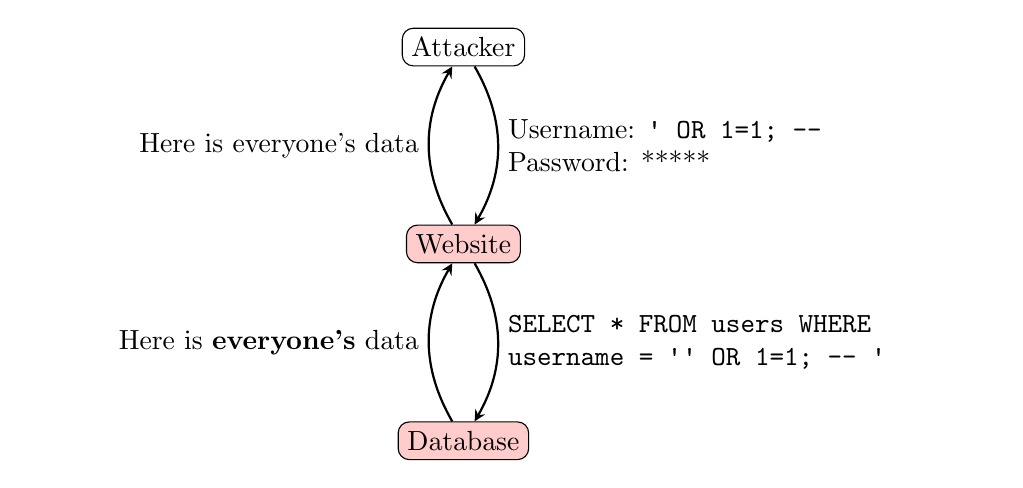
\begin{tikzpicture}[node distance=2.5cm]
  \node (user) [plain] {Attacker};
  \node (webserver) [trusted, below of=user] {Website};
  \node (database) [trusted, below of=webserver] {Database};

  \draw [arrow, bend left] (user) edge node[right] {\parbox{0.5\textwidth}{Username: \texttt{\textquotesingle \ OR 1=1; --} \\ Password: *****}} (webserver);

  \draw [arrow, bend left] (webserver) edge node[right] {\parbox{0.5\textwidth}{\raggedright \texttt{SELECT * FROM users WHERE \\ username = \textquotesingle\textquotesingle \ OR 1=1; -- \textquotesingle}}} (database);

  \draw [arrow, bend left] (database) edge node[left] {\parbox{0.4\textwidth}{\hfill Here is \textbf{everyone's} data}} (webserver);
  \draw [arrow, bend left] (webserver) edge node[left] {\parbox{0.4\textwidth}{\hfill Here is everyone's data}} (user);        
\end{tikzpicture}

\subsection{Project Summary}
This project aims to produce an authentication system for web applications, such that a user can authenticate to a web application using a Kerberos ticket and the web application can use this ticket to obtain the user's data from a database. The overall structure of the authentication process is as shown below, noting that the application itself does not have any other access means of accessing the database, so an attack such as the one depicted above cannot take place.

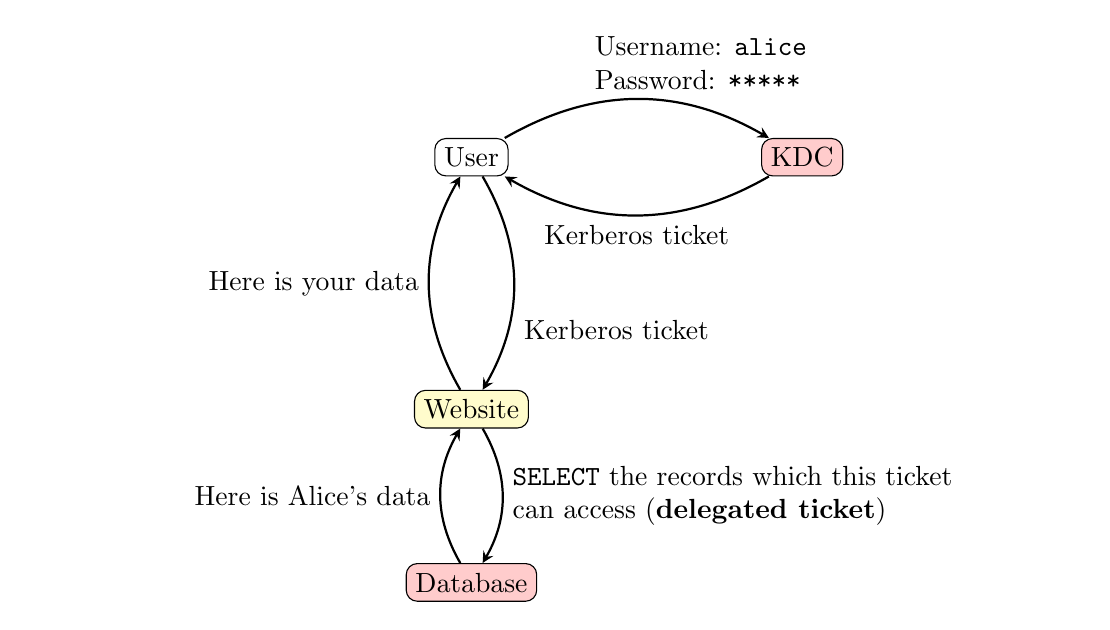
\begin{tikzpicture}[node distance=2.2cm]
  \node (user) [plain] {User};
  \node (webserver) [untrusted, below of=user, yshift=-1cm] {Website};
  \node (database) [trusted, below of=webserver] {Database};
  \node (kdc) [trusted, right of=user, xshift=2cm] {KDC};

  \draw [arrow, bend left] (user) edge node[above, xshift=2.5cm] {\parbox{0.5\textwidth}{Username: \texttt{alice} \\ Password: \texttt{*****}}} (kdc);

  \draw [arrow, bend left] (kdc) edge node[above, yshift=-0.5cm] {Kerberos ticket} (user);

  \draw [arrow, bend left] (user) edge node[right, yshift=-0.6cm] {Kerberos ticket} (webserver);

  \draw [arrow, bend left] (webserver) edge node[right] {\parbox{0.5\textwidth}{\raggedright \texttt{SELECT} the records which this ticket can access (\textbf{delegated ticket})}} (database);

  \draw [arrow, bend left] (database) edge node[left] {\parbox{0.4\textwidth}{\hfill Here is Alice's data}} (webserver);
  \draw [arrow, bend left] (webserver) edge node[left] {\parbox{0.4\textwidth}{\hfill Here is your data}} (user);        
\end{tikzpicture}


\section{Preparation}

\subsection{Kerberos}
The Kerberos protocol works based on a system of \textit{tickets}, which are managed by a \textit{Key Distribution Centre} (KDC). The basic requirement of the system is to allow a centralised database of users (for example, the main login directory in an office) who can demonstrate their identity in order to log in to applications and services, but \textit{without} having to store or transmit passwords or other long-term secrets on potentially untrusted machines.

The basic workings of the protocol are as follows:

\begin{itemize}
\item
  A user initiates a session by reqesting a Kerberos ticket from the KDC, authenticating using their password.
\item
  The KDC returns a \textit{ticket-granting ticket} (TGT), and returns it encrypted using the user's password.
\item
  The user decrypts the TGT, and the user's machine can then discard the stored password.
\item
  When the user wants to access a service, they send the TGT back to the KDC along with an identifier for the service which they want to use.
\item
  The TGT grants the user a \textit{service ticket}, which the user then passes on to the service. The service is then able to use that ticket for authentication.
\item
  (Extend to cover ticket delegation here)
\end{itemize}

\section{Implementation}

\subsection{Implementing SQL Procedures}
As one aspect of the project, the database server must be able to provide the correct set of records to each user without exposing the rest of the table. Since PostgreSQL does not offer the ability to selectively allow a user to query certain rows in a table, this can instead be acheived using stored procedures. However, these are not a standardised construct in SQL, and even within PostgreSQL there are multiple ways to achieve this.

\subsubsection{\texttt{SECURITY DEFINER} functions}
A PostgreSQL function with \texttt{SECURITY DEFINER} in the signature runs ``as'' the user creating the function, regardless of who executes it\cite{postgres-SEC_DEF} (in a similar way to how the \texttt{setuid} bit works in Unix). This allows the database owner to create a function which can read the whole table and when run, perform some check based on the user calling it and return appropriate results.

This approach requires some caution since the \texttt{SECURITY DEFINER} property also redefines the \verb+current_user+ variable (which normally contains the username of the user executing a query) to the user who defined the function, although this can be worked around using \verb+session_user+ instead. It is also not as easily integratable into frameworks such as Django, which are designed to execute queries on tables rather than (effectively) making function calls to an API.

\subsubsection{Use of \texttt{ON SELECT} to redefine selection}
PostgreSQL also allows rules to be created which effectively redefine actions on tables. For example, a rule could be used to replace the default \texttt{SELECT} rule on the table storing file information with one that checked user permissions.

However, this is likely to introduce unnecessary complexity (particularly with ensuring that administrators can still access data as necessary, for example). For these reasons, the PostgreSQL documentation considers it ``better style to write a \texttt{CREATE VIEW} command than to create a real table and define an \texttt{ON SELECT} rule for it''\cite{postgres-CREATE_RULE}.

\subsubsection{SQL views}
These effectively allow a new table to be created out of a view over an existing table. Using syntax such as the following, it is therefore possible to construct a new table which only has the calling user's files visible; the user can then be granted access to this view (which automatically selects files based on their own username) and does not then need to have any access to the original table. For web application purposes, it can be queried just like any other table.

\begin{verbatim}
CREATE VIEW my_files AS
SELECT f.*
FROM files_file f, files_permission p
WHERE f.id = p.file_id
AND p.owner = user;
\end{verbatim}

\section{Evaluation}

\section{Conclusion}

\section*{Bibliography}
\begin{thebibliography}{9}
\bibitem{OWASP10} OWASP \textit{Top 10 Web Application Security Risks} list. \url{https://owasp.org/www-project-top-ten/} (accessed 21/10/2020)

\bibitem{GDPR} Data Protection Act 2018: Section 157 \url{https://www.legislation.gov.uk/ukpga/2018/12/section/157/enacted} (accessed 10/02/2021)

\bibitem{postgres-SEC_DEF} PostgreSQL documentation: \texttt{CREATE FUNCTION} \url{https://www.postgresql.org/docs/current/sql-createfunction.html#SQL-CREATEFUNCTION-SECURITY} (accessed 22/02/2021)

\bibitem{postgres-CREATE_RULE} PostgreSQL documentation: \texttt{CREATE RULE} \url{https://www.postgresql.org/docs/current/sql-createrule.html} (accessed 22/02/2021)
\end{thebibliography}


\end{document}
